\chapter{宇宙与地球中的元素}\label{ch:g9:elements-universe-earth}

你骨骼中的钙、血液中的铁，以及你呼吸的氧，
都不是在地球上形成的。它们是在太阳诞生之前，
在已经诞生又陨灭的恒星内部形成的，此后数十亿年间，它们从岩石到海洋，
从海洋到植物，从植物到动物。有些元素无处不在，
另一些则十分稀少。哪些元素构成了恒星、
地球、海洋，以及我们自己？

\begin{recall}
化学元素是具有相同\omterm{def:g9:inside-the-atom:atomic-number}{原子序数} $Z$ 的一类\omterm{def:g7:atoms-and-molecules:atom}{原子}，
\omterm{def:g7:atoms-and-molecules:atom}{原子}的质量约为 $A \times \qty{1.67e-27}{kg}$，其中 $A$
为\omterm{def:g9:inside-the-atom:atomic-number}{质量数}（见\cref{ch:g9:inside-the-atom}）。\omterm{def:g9:periodic-table-first-look:periodic-table}{元素周期表}
按\omterm{def:g9:inside-the-atom:atomic-number}{原子序数}列出了 118 种元素
（见\cref{ch:g9:periodic-table-first-look}）。\omterm{def:g4:air-a-mixture-of-gases:air}{空气}中约五分之四是
氮气，五分之一是氧气（见\cref{ch:g4:air-a-mixture-of-gases}）。
\end{recall}

\section{恒星中的元素}

\begin{definition}[丰度]\label{def:g9:elements-universe-earth:abundance}
元素在一个物质体系中的\emph{丰度}\index{丰度}，
即该元素在该体系中——如恒星、地壳、海洋或生物体——
所占总质量的比例，通常以百分数表示。
\end{definition}

\begin{proposition}[太阳由氢和氦组成]\label{prop:g9:elements-universe-earth:sun}
% ledger: ab:sun-X, ab:sun-Y, ab:sun-Z
按质量计，太阳表面约有 \qty{74}{\percent} 为氢，
\qty{25}{\percent} 为氦，其余元素合计仅约 \qty{1.3}{\percent}。
宇宙中大部分可见物质的组成与之相似，
主要是氢和氦，
其余元素只占一小撮。
\end{proposition}

\begin{proposition}[恒星中形成的元素]\label{prop:g9:elements-universe-earth:stars}
氢和大部分氦形成于宇宙诞生后的最初几分钟。
几乎所有较重的元素——碳、氧、铁、金——
则是后来在恒星内部制造出来的，恒星爆炸时将其抛散到太空中。
新的恒星和行星正是由富集了这些重元素的尘埃形成的。
恒星如何做到这一点，在 One Physics Book 中有介绍。
\end{proposition}

\begin{omfigure}
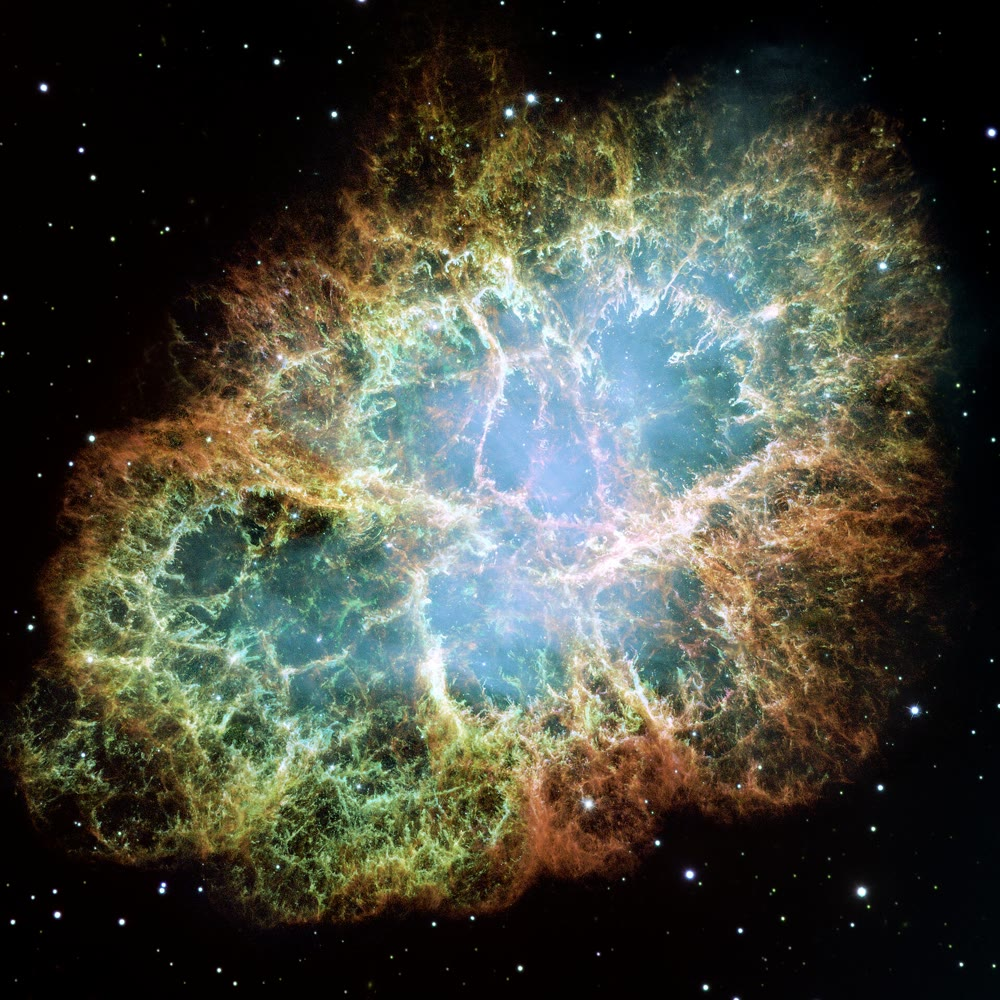
\includegraphics[width=0.45\linewidth]{images/book1/crab-nebula.jpg}

{\small 蟹状星云，是一颗近千年前爆炸的恒星所留下的云团，
将新的元素散布到太空中
（照片：NASA、ESA、J.~Hester 与 A.~Loll）。}
\end{omfigure}

\section{地球}

\begin{proposition}[地壳]\label{prop:g9:elements-universe-earth:crust}
% ledger: ab:crust-O, ab:crust-Si, ab:crust-Al, ab:crust-Fe, ab:crust-Ca, ab:crust-Na, ab:crust-K, ab:crust-Mg, ab:crust-first10
地球表面那层薄薄的岩石外壳即地壳，按质量计，氧几乎占一半，
硅占四分之一以上：岩石和沙子主要是硅与少数\omterm{def:g9:periodic-table-first-look:metal}{金属}的氧化物。
八种元素——氧、硅、
铝、铁、钙、钠、钾、镁——合计约占
\qty{99}{\percent}。氢和氦在恒星中十分常见，
但在地壳中很稀少：这些轻质气体早已从年轻的地球上逸散。
\end{proposition}

\begin{remark}[地球内部]\label{rem:g9:elements-universe-earth:core}
地壳并不是地球的全部。铁密度大，
在年轻的地球处于熔融状态时向中心下沉：地核主要由铁构成，
并含有一些镍。
\end{remark}

\begin{proposition}[海洋与空气]\label{prop:g9:elements-universe-earth:ocean}
% ledger: sea:salts-share, sea:NaCl-ions, sea:MgSO4-ions, air:N2, air:O2
海水主要是水，即由氢和氧组成的水，
另含\omterm{def:g2:mixing-and-dissolving:dissolve}{溶解}盐约 \qty{3.5}{\percent}（按质量计）。在\omterm{def:g2:mixing-and-dissolving:dissolve}{溶解}的\omterm{def:g9:ions:ion}{离子}中，
氯\omterm{def:g9:ions:ion}{离子}和钠\omterm{def:g9:ions:ion}{离子}约占 \qty{85}{\percent}，
镁\omterm{def:g9:ions:ion}{离子}和硫酸根\omterm{def:g9:ions:ion}{离子}又占 \qty{10}{\percent}。
\omterm{def:g4:air-a-mixture-of-gases:air}{空气}主要是氮气和氧气。
\end{proposition}

\begin{omfigure}
\begin{tikzpicture}
\begin{axis}[xbar, width=0.40\linewidth, height=5.4cm, xmin=0, xmax=85,
    bar width=7pt, symbolic y coords={Mg,K,Na,Ca,Fe,Al,Si,O}, ytick=data,
    xlabel={质量百分数}, title={\small 地壳},
    nodes near coords, nodes near coords style={font=\scriptsize},
    tick label style={font=\small}, label style={font=\small},
    axis lines*=left, enlarge y limits=0.08]
% ledger: ab:crust-O, ab:crust-Si, ab:crust-Al, ab:crust-Fe, ab:crust-Ca, ab:crust-Na, ab:crust-K, ab:crust-Mg
\addplot[fill=omDef!45, draw=omDef] coordinates {(46.6,O) (27.7,Si) (8.1,Al)
  (5.0,Fe) (3.6,Ca) (2.8,Na) (2.6,K) (2.1,Mg)};
\end{axis}
\end{tikzpicture}\hfill
\begin{tikzpicture}
\begin{axis}[xbar, width=0.40\linewidth, height=5.4cm, xmin=0, xmax=85,
    bar width=7pt, symbolic y coords={{P},{N},{Ca},{H},{C},{O}}, ytick=data,
    xlabel={质量百分数}, title={\small 人体},
    nodes near coords, nodes near coords style={font=\scriptsize},
    tick label style={font=\small}, label style={font=\small},
    axis lines*=left, enlarge y limits=0.1]
% ledger: body:atoms-O, body:atoms-C, body:atoms-H, body:atoms-N, body:atoms-Ca, body:atoms-P (masses = atoms x atomic mass, over 70 kg)
\addplot[fill=omProp!45, draw=omProp] coordinates {(61.1,O) (22.9,C) (10.1,H)
  (1.3,N) (1.5,Ca) (0.7,P)};
\end{axis}
\end{tikzpicture}

{\small 按质量计的\omterm{def:g9:elements-universe-earth:abundance}{丰度}。左图：地壳中的八种主要元素；右图：
瘦成年人体中的六种主要元素。
（根据估计的\omterm{def:g7:atoms-and-molecules:atom}{原子}数计算得出）。}
\end{omfigure}

\section{人体}

\begin{proposition}[我们由什么构成]\label{prop:g9:elements-universe-earth:body}
% ledger: body:atoms-O, body:atoms-C, body:atoms-H, body:atoms-N, body:atoms-Ca, body:atoms-P, body:atoms-total
按质量计，瘦成年人体中约有 \qty{61}{\percent} 的氧、
\qty{23}{\percent} 的碳和 \qty{10}{\percent} 的氢——主要存在于
水和生命\omterm{def:g7:atoms-and-molecules:molecule}{分子}中——其次是氮、钙（存在于
骨骼和牙齿中）以及磷。若按\omterm{def:g7:atoms-and-molecules:atom}{原子}数而非质量计，
顺序会发生变化：人体中氢\omterm{def:g7:atoms-and-molecules:atom}{原子}的个数比所有
其他\omterm{def:g7:atoms-and-molecules:atom}{原子}加起来还多，因为氢\omterm{def:g7:atoms-and-molecules:atom}{原子}非常轻。质量为
\qty{70}{kg} 的人体约含 $7 \times 10^{27}$ 个\omterm{def:g7:atoms-and-molecules:atom}{原子}。
\end{proposition}

\begin{method}[读丰度图]\label{met:g9:elements-universe-earth:read}
\begin{enumerate}
  \item 查看测量的是什么：质量（多数图）或\omterm{def:g7:atoms-and-molecules:atom}{原子}数。
  \item 读出每种元素所占的份额，将主要元素的份额相加，
        看它们合计占多少。
  \item 比较两个人体时，找出二者共有的元素，
        以及只在其中一者中出现的元素。
\end{enumerate}
氧在本章两张图中都居首位：按质量计，它是地壳
和人体中最常见的元素。
\end{method}

\section{同一批原子，循环利用}

\begin{example}[一个碳原子的旅程]\label{ex:g9:elements-universe-earth:journey}
一个碳\omterm{def:g7:atoms-and-molecules:atom}{原子}在很久以前的恒星中形成，之后可以在
石灰岩中停留数百万年，经火山释放为二氧化碳，再被
一片叶子吸收，成为果实中糖的一部分，进入
食用这果实的动物体内，最后又以二氧化碳的形式呼出。\omterm{def:g7:atoms-and-molecules:atom}{原子}
不会因\omterm{def:g5:irreversible-changes:chemical-change}{化学变化}而被破坏，它们只是被传递下去。
\end{example}

\begin{omfigure}
\begin{tikzpicture}[font=\small,
    box/.style={draw=omDef, fill=omDef!6, rounded corners=2pt, align=center,
      minimum height=0.85cm, text width=2.3cm}]
  \node[box] (a) at (0,2.2) {岩石中 \\（石灰岩）};
  \node[box] (b) at (4.3,2.2) {空气中 \\（\ce{CO2}）};
  \node[box] (c) at (8.6,2.2) {叶片中 \\（糖）};
  \node[box] (d) at (8.6,0) {动物体内};
  \node[box] (e) at (4.3,0) {呼出 \\（\ce{CO2}）};
  \draw[->, thick, omProp] (a) -- node[above, font=\footnotesize] {火山} (b);
  \draw[->, thick, omProp] (b) -- (c);
  \draw[->, thick, omProp] (c) -- node[right, font=\footnotesize] {被食用} (d);
  \draw[->, thick, omProp] (d) -- (e);
  \draw[->, thick, omProp] (e) -- (b);
\end{tikzpicture}

{\small 一个碳\omterm{def:g7:atoms-and-molecules:atom}{原子}从岩石进入\omterm{def:g4:air-a-mixture-of-gases:air}{空气}，再进入叶片、动物体内，最后回到
\omterm{def:g4:air-a-mixture-of-gases:air}{空气}中：\omterm{def:g7:atoms-and-molecules:atom}{原子}本身从未被破坏。}
\end{omfigure}

\begin{omfigure}
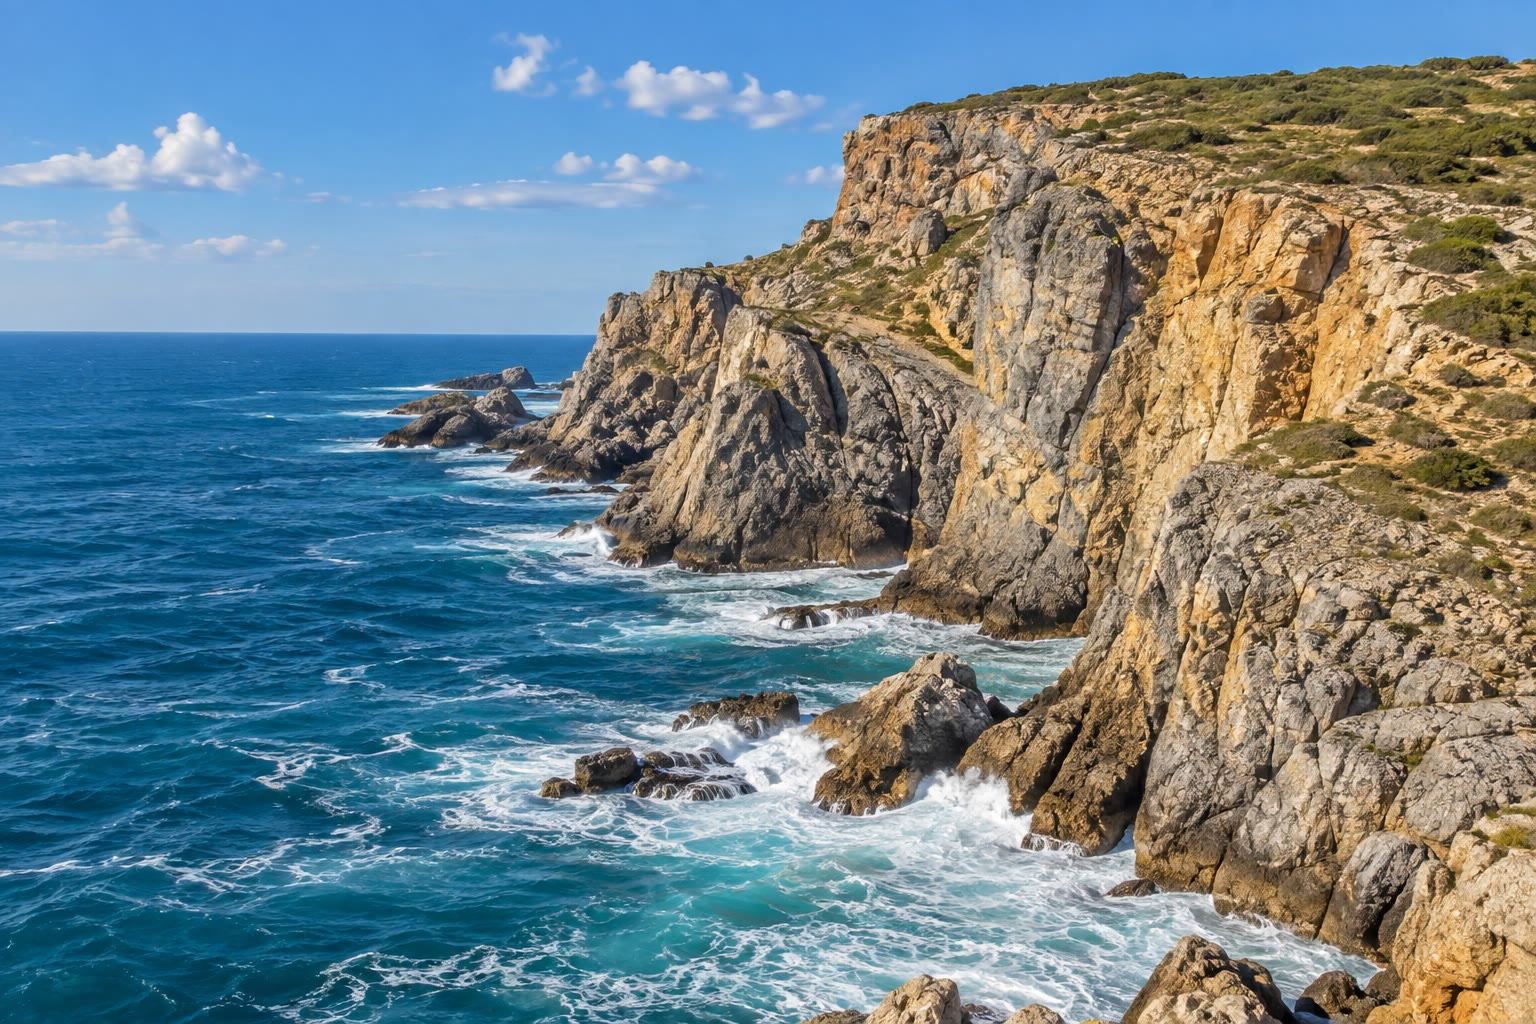
\includegraphics[width=0.55\linewidth]{images/book1/ai/g9-coastal-cliff.jpg}

{\small 岩石、海水和\omterm{def:g4:air-a-mixture-of-gases:air}{空气}：由相同元素组成的三种
截然不同的\omterm{def:g6:pure-substances-and-mixtures:mixture}{混合物}。}
\end{omfigure}

\section{练习}

\begin{exercise}[$\star$]\label{exo:g9:elements-universe-earth:1}
太阳的绝大部分由哪两种元素组成？
\end{exercise}

\begin{exercise}[$\star$]\label{exo:g9:elements-universe-earth:2}
哪种元素在地壳中含量最多？在人体中（按质量计）
含量最多的又是哪种元素？
\end{exercise}

\begin{exercise}[$\star$]\label{exo:g9:elements-universe-earth:3}
比氦重的大多数元素是在哪里形成的？
\end{exercise}

\begin{exercise}[$\star$]\label{exo:g9:elements-universe-earth:4}
海水质量中，\omterm{def:g2:mixing-and-dissolving:dissolve}{溶解}的盐占百分之多少？
\end{exercise}

\begin{exercise}[$\star\star$]\label{exo:g9:elements-universe-earth:5}
利用地壳的图，将氧和硅的份额相加。
大致占地壳的多大比例？
\end{exercise}

\begin{exercise}[$\star\star$]\label{exo:g9:elements-universe-earth:6}
为什么地壳中的氢和氦如此之少，
而太阳几乎完全由它们构成？
\end{exercise}

\begin{exercise}[$\star\star$]\label{exo:g9:elements-universe-earth:7}
一个质量为 \qty{70}{kg} 的人体，其中碳
占 \qty{23}{\percent}，碳的质量为多少？
\end{exercise}

\begin{exercise}[$\star\star$]\label{exo:g9:elements-universe-earth:8}
为什么按质量计氧是人体中含量最多的元素，
而按\omterm{def:g7:atoms-and-molecules:atom}{原子}数计氢才是最多的？
\end{exercise}

\begin{exercise}[$\star\star$]\label{exo:g9:elements-universe-earth:9}
一块 \qty{1000}{kg} 的花岗岩是地壳的典型样品，
利用图中数据，大约含有多少质量的铝？
\end{exercise}

\begin{exercise}[$\star\star$]\label{exo:g9:elements-universe-earth:10}
哪些元素既是地壳的主要元素，
又是人体的主要元素？
\end{exercise}

\begin{exercise}[$\star\star\star$]\label{exo:g9:elements-universe-earth:11}
一个 \qty{70}{kg} 的人体约含钙 \qty{1.06}{kg}。求
一个钙\omterm{def:g7:atoms-and-molecules:atom}{原子}的质量（$A = 40$），然后求钙\omterm{def:g7:atoms-and-molecules:atom}{原子}的个数。
用科学记数法表示。
\end{exercise}

\begin{exercise}[$\star\star\star$]\label{exo:g9:elements-universe-earth:12}
你体内的\omterm{def:g7:atoms-and-molecules:atom}{原子}此前都曾是其他事物的一部分。用
一个碳\omterm{def:g7:atoms-and-molecules:atom}{原子}的历程，解释地球上碳\omterm{def:g7:atoms-and-molecules:atom}{原子}的
总数为何几乎不变。
\end{exercise}

\section{问题：我身体里有多少个原子？}

\begin{problem}[{周末问题——从丰度图到
人体中氧原子的个数}]
\label{pb:g9:elements-universe-earth:1}
% ledger: body:atoms-O, body:atoms-total
一名体型偏瘦、质量为 \qty{70}{kg} 的成年人，按质量计约含
\qty{61}{\percent} 的氧、\qty{23}{\percent} 的碳和 \qty{10}{\percent} 的氢。
取一个\omterm{def:g9:inside-the-atom:proton}{核子}的质量为 \qty{1.67e-27}{kg}；一个氧\omterm{def:g7:atoms-and-molecules:atom}{原子}有 16 个\omterm{def:g9:inside-the-atom:proton}{核子}，
一个碳\omterm{def:g7:atoms-and-molecules:atom}{原子}有 12 个\omterm{def:g9:inside-the-atom:proton}{核子}，一个氢\omterm{def:g7:atoms-and-molecules:atom}{原子}有 1 个\omterm{def:g9:inside-the-atom:proton}{核子}。\omterm{def:g9:inside-the-atom:nucleus}{电子}忽略不计。

\medskip
\noindent\textbf{第一部分——质量。}
\begin{enumerate}
  \item 求人体中氧的质量。
  \item 求碳和氢的质量。
  \item 这三种元素合计
        占总质量的百分之几？
  \item 这些氧和氢大部分存在于同一种化合物中。该化合物是什么？
\end{enumerate}

\medskip
\noindent\textbf{第二部分——一个\omterm{def:g7:atoms-and-molecules:atom}{原子}。}
\begin{enumerate}[resume]
  \item 求一个氧\omterm{def:g7:atoms-and-molecules:atom}{原子}的质量。
  \item 求一个碳\omterm{def:g7:atoms-and-molecules:atom}{原子}和一个氢\omterm{def:g7:atoms-and-molecules:atom}{原子}的质量。
  \item 多少个氢\omterm{def:g7:atoms-and-molecules:atom}{原子}的质量与一个氧\omterm{def:g7:atoms-and-molecules:atom}{原子}的质量相等？
  \item 为什么可以忽略\omterm{def:g9:inside-the-atom:nucleus}{电子}？
\end{enumerate}

\medskip
\noindent\textbf{第三部分——计数。}
\begin{enumerate}[resume]
  \item 求人体中氢\omterm{def:g7:atoms-and-molecules:atom}{原子}的个数。
  \item 求碳\omterm{def:g7:atoms-and-molecules:atom}{原子}的个数。
  \item 求人体中氧\omterm{def:g7:atoms-and-molecules:atom}{原子}的个数。
  \item 仔细估算表明，这样的人体中约含 $1.61 \times 10^{27}$
        个氧\omterm{def:g7:atoms-and-molecules:atom}{原子}。将结果与你的计数比较，并用两位有效数字写出
        \qty{70}{kg} 人体中氧\omterm{def:g7:atoms-and-molecules:atom}{原子}的个数。
\end{enumerate}
\end{problem}
